\chapter{Theoretical background}
\label{chapter:theoretical_bg}
\section{Computer vision tasks}
\begin{figure}
    \centering
    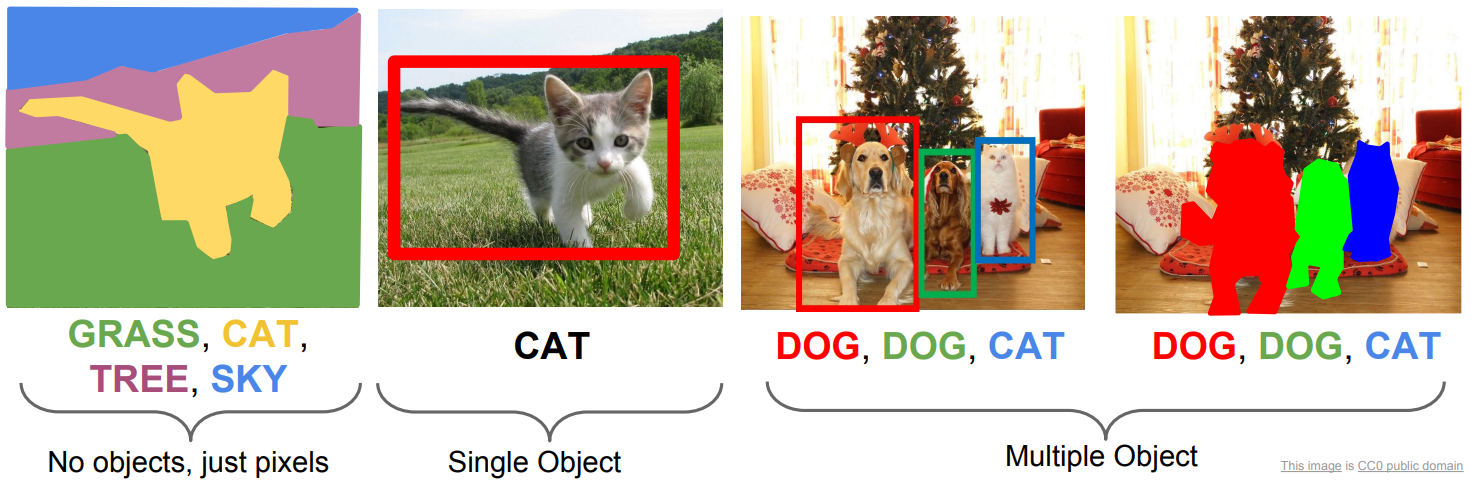
\includegraphics[width=\linewidth]{images/computer_vision_tasks.png}
    \caption{From the left: semantic segmentation, object localization, object detection, instance segmentation}.
    \label{fig:computer_vision_tasks}
\end{figure}
This section provides a brief overview of standard computer vision tasks.
\subsection{Classification}
Let's say we have an image $\mathbf{x}$. In a classification task, our goal is to assign one of $n$ possible classes to the image:
\begin{align}
    \hat{y} = f_\theta\left(\mathbf{x} \right),
\end{align}
where $f$ is a mapping, sometimes called a model, and $\theta$  represents model parameters if it holds that $\hat{y}=y$, where $y$ is a true class of the image $\mathbf{x}$, the classification is considered to be correct.
It is possible to output $\mathbf{p} \in \mathbb{R}^n$ instead of $\hat{y}$, where $p_i \in \mathbf{p}$ is probability of $i = y$, modeled by $f_\theta$.

\subsection{Semantic segmentation}
For an input image $x \in \mathbb{R}^{n \times m}$, the goal is to output $\mathbf{\hat{Y}} \in \mathbb{R}^{n \times m}$, where $\hat{y_{i,j}}$ is the predicted class of pixel $i,j$ in image $\mathbf{x}$. Similarly to the classification problem, we can output matrix $\mathbf{P} \in \mathbb{R}^{n \times m \times c}$, where $p_{i,j,c}$ is the probability of $pixel_{i,j}$ belonging to class $c$. A sample of semantic segmentation output can be seen in Figure \ref{fig:computer_vision_tasks}.

\subsection{Object detection}
\label{subsec:object_detection}
In object detection, the goal is to locate and recognize objects of interest in image $\mathbf{x}$. A rectangle and a category represent a ground truth object. Model predicts $\mathbf{Y} \in \mathbb{R}^{n \times 6}$ values for each image. Each row of $\mathbf{Y}$ consists of four numbers, which describe a rectangle, the category of the object inside the rectangle, and a number in the range from 0 to 1 called the confidence. In literature, we can see the term score instead of confidence. Nevertheless, the meaning remains the same: Certainty of the network regarding the particular prediction described by the bounding box and category. Please note that the confidence of predictions does not sum to one. In other words, we are not talking about probabilities since multiple detections per image can correspond to the ground truth.

\subsection{Instance segmentation}
Instance segmentation is similar to semantic segmentation, with the alteration saying that two objects of the same category would have different ground truth values. If we have $\mathcal{O}_1, \mathcal{O}_2$, where $\mathcal{O}_i \subset \mathbf{x}$ are pixels of object $i$ in image $\mathbf{x}$. Then
\begin{align}
    o_{1_i} \neq o_{2_i} \quad \text{for} \quad o_{1_i} \in \mathcal{O}_1, o_{2_i} \in \mathcal{O}_2;\forall i.
\end{align}

\section{Data format in object detection}
As described in Section \ref{subsec:object_detection}, the position of an object is denoted by a bounding box.  The four parameters used to describe a bounding box can be selected in multiple ways. This ambiguity led to a disjoint notation. The most widespread are as follows.
\subsection{PASCAL VOC}
The format was introduced together with the PASCAL VOC dataset, the most popular dataset for object detection algorithm benchmarking in 2010. The bounding box is described by points $p_1(x,y),p_2(x,y)$ located in the top-left and bottom right corner. The coordinates range from 0 to image width/height in pixels. All the annotations are stored in a single XML file \cite{Everingham2009,Padilla2021}.
\subsection{COCO}
COCO data format is represented by a single JSON file containing all bounding boxes of the dataset. The boxes are described by the top-left corner point $p(x,y)$ and the width and height of the box. The coordinates and box dimensions are again in the range 0 to image dimensions. In MS COCO, the annotation can be accompanied by a piece of additional information to solve the task as an instance segmentation problem.
\subsection{YOLO}
This format was introduced together with the first YOLO architecture \cite{Redmon2015}, and this annotation style is still persistent whenever working with the YOLO-family neural networks.
In this format, the annotations are divided into multiple TXT files and each of them contains annotations for a single image.
The bounding box is described similarly as in the COCO dataset, but the coordinates are normalized to be in the 0 to 1 range. The advantage of this approach is that the annotations do not have to be modified when image dimensions are scaled \cite{Redmon2015, Padilla2021}.


\section{Metrics}
\subsection{Intersection over union (IOU) }
Intersection over union, also known as the Jaccard index, is defined as demonstrated: Let $B_{gt}$ and $B_p$ be a ground truth and a predicted bounding box. The Jaccard index $J$ is calculated as
\begin{align}
    IOU = J(B_p, B_{gt}) = \frac{area(B_p \bigcap B_{gt})}{area(B_p \bigcup B_{gt})}.
    \label{eq:iou}
\end{align}
From the Equation \ref{eq:iou}, we can observe that the lowest value of IOU is 0. This means there is no overlap and the maximal value is 1, indicating a perfect match.
We use a predefined threshold value of IOU to decide if the predicted bounding box matches the ground truth. Usually, we choose this threshold to be 0.5 or above.

IOU can be defined for the semantic segmentation task with two classes (e.g. background and target class). Let $\mathbb{\hat{Y}} \in \mathbb{R}^{m \times n}$ be the mask of the predicted values, where $\hat{y}_{i,j} = 1$ if the model predicts, that pixel $i,j$ belongs to target class. The IOU is defined as:
\begin{align}
    IOU = \frac{\sum_{i=1}^{m} \sum_{j=1}^{n} \hat{y}_{i,j} \wedge  y_{i,j}}{\sum_{i=1}^{m} \sum_{j=1}^{n} \hat{y}_{i,j} \vee  y_{i,j}},
\end{align}
where $y_{i,j} \in \mathbf{Y} \in \mathbb{R} ^ {m \ times n}$ is the ground truth value for pixel $i,j$.


\begin{figure}
    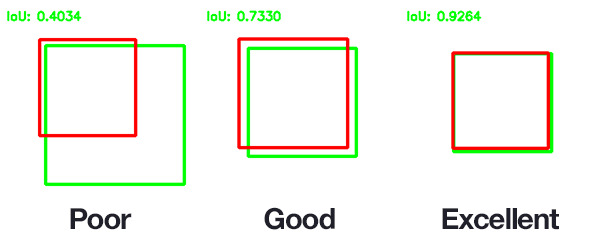
\includegraphics[width = 0.9\linewidth]{images/IOU.jpg}
    \caption{Examples of IOUs for different overlaps between GT and predicted box, source. \cite{Cowton2019}}
    \label{fig:iou}
\end{figure}

\subsection{Precision and recall}
\subsubsection{Precision}
\label{subsec:precision}
When speaking about object detection, we say that a prediction is a true positive (TP) if the IOU value is greater than the predefined threshold $\tau$. If otherwise, the prediction is treated as a false positive (FP). Let's assume there are N predictions of our model, from which S are correct. Precision is defined as
\begin{align}
    Precision(\tau, \gamma) = \frac{TP(\tau, \gamma)}{TP(\tau, \gamma) + FP(\tau, \gamma)},
\end{align}
where $\gamma$ is the confidence threshold, meaning we discard all predictions with confidence smaller than $\gamma$. Note that for fixed value of $\tau$ are $FP(\gamma)$ and $TP(\gamma)$ decreasing functions of $\gamma$ \cite{Padilla2021}.

\

\subsubsection{Recall}
\label{subsec:recall}
If there is a ground truth bounding box for which there are no given detection values of $\gamma$ and $\tau$, we say it is a false negative (FN). If we consider a dataset with G ground-truths and N predictions of which S is correct, where $(S \leq G)$, the recall is expressed as:
\begin{align}
    Recall(\tau, \gamma) = \frac{TP(\tau, \gamma)}{ TP(\tau, \gamma) + FN(\tau, \gamma)}.
    \label{eq:recall}
\end{align}
Since the value of $FN(\gamma)$ increases with the growing value of $\gamma$, we see that recall is the decreasing function of $\gamma$.

\subsubsection{F1 score}
The value of the F1 score is computed as the harmonic mean of precision and recall.
\begin{align}
    F1(\tau, \gamma) = \frac{2 \cdot Recall(\tau,\gamma) \cdot Precision(\tau, \gamma)}{Recall(\tau,\gamma) + Precision(\tau, \gamma)}.
\end{align}

\subsubsection{Precision-recall curve (PR curve)}
From Subsections \ref{subsec:precision} and \ref{subsec:recall}, we were able to observe that precision mainly grows as we increase the confidence threshold $\gamma$, while at the same time recall decreases. The precision-recall curve captures the relation between precision and recall. An example of the curve is illustrated as the blue line in Figure \ref{fig:pr_curve}. In other words, we can say that the precision-recall curve is a mapping
\begin{align}
    \gamma \rightarrow Precision(\gamma) \times  Recall(\gamma),
    \label{eq:pr_curve}
\end{align}
where $\gamma$ ranges from 1 to 0.

\subsubsection{Mean average precision (mAP)}
To calculate mAP we first need to get the PR-curve and then interpolate the precision values. Suppose that we have $K$ different confidence values $\gamma$ among model predictions, which are ordered as
\begin{align}
    \gamma(k),\: k = 1,2,...,K,  \; \text{such that } \gamma(i) > \gamma(j) \: for \: i > j.
\end{align}
The interpolated precision-recall curve is then defined as
\begin{align}
    Precision_{interp}(R) = \max_{k|Recall(\gamma(k)) \geq R} \{  Precision(\gamma(k)) \},
\end{align}
where $R$ is a real value contained in interval [0,1] \cite{Padilla2021}.
The interpolated precision-recall curve is pictured in Figure \ref{fig:pr_curve} in red color. Now, we can compute the average precision (AP) as the area under the interpolated PR curve.
In practice, there are two different ways to approach the Reimann integral. They differ in the number of samples used to compute the integral and are called N-point and all-point interpolation. The N-point, specifically 101 point interpolation, is used in the MS COCO competition. On the other hand, the all-point interpolation is nowadays used in PASCAL VOC challenges \cite{Padilla2020, Padilla2020}.

Since the AP is calculated per class, the mean average precision is defined as the average in all categories.

In Subsections \ref{subsec:precision} and \ref{subsec:recall}, we stated that precision and recall depend on a predefined IOU threshold $\tau$ to consider prediction as true positive. This dependency makes the value of MAP vary over different values of $\tau$. The threshold value used for computation of the mAP is usually denoted in the metrics name, such as $AP@.5$ in the case of MS COCO. \footnote{Note that even though the mean average precision is computed, the $AP$ shortcut, which stands for average precision, is used.} The standalone $AP$ without any numerical values attached to it usually refers to the official COCO metric. The official COCO metric is in its explicit form written as $AP@[.5:0.05:0.95]$ and is computed as the average of MAP values for ten different $\tau$ values, ranging from 0.5 to 0.95.

The letters S, M,  and L in the subscript, such as $AP_S$ denote that the metrics are calculated for a subset of ground truth predictions only. Taking into the consideration only bounding boxes with area $\leq 32^2$ pixels, $32^2 \le $ area $ \leq 96^2$ pixels and area $> 96^2$ pixels

\subsection{Mean average recall in MS-COCO (mAR)}
PyCOCOtools, the official metrics for MS-COCO benchmark \cite{pycocotools}, compute the average recall (AR) by the following approach: Predictions are sorted according to their confidence in a decreasing order. We take $n$ boxes with the highest confidence values and evaluate their recall by Equation \ref{eq:recall} for a predefined IOU threshold $\theta$. We use a similar notation as in the case of AP, where $AR@.X_{na}$ denotes the average recall computed for IOU threhsold $X$, where we consider $n$ most confident predictions. By $a \in \{ S, M, L, \text{all} \}$ we denote size of the rectangles, for which AR is computed. If we omit some of those, the following default values are used $a=\text{all}, n = 100, X = [.5:0.05:0.95]$.

\begin{figure}
    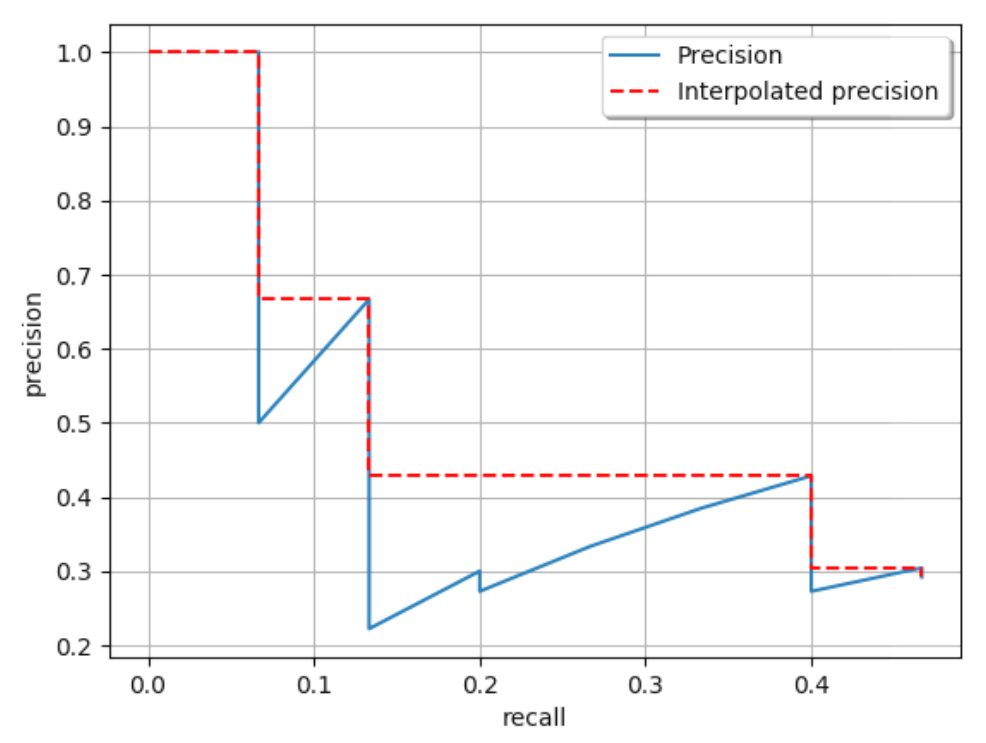
\includegraphics[width = 0.78\linewidth]{images/PR-curve.png}
    \caption{Standard and interpolated precision-recall curve, source \cite{Padilla2020}}
    \label{fig:pr_curve}
\end{figure}


\subsubsection{Cross-Entropy loss}
\label{sec:cross_entropy}
Let $\mathbf{y} \in \mathbb{R}^n, y_i \in \{ 0, 1 \}$ be a vector of ground truth classes and $\hat{\mathbf{y}} \in \mathbb{R}^n$ be a vector of model preditions, where $\hat{y_i} \in [0, 1]$ is the predicted probability, that $i_{th}$ element belongs to class $1$. The cross-entropy loss is computed as follows \cite{Jadon2020}:
\begin{align}
    L_{CE}(\mathbf{y}, \hat{\mathbf{y}}) = - \frac{1}{N} \sum_{i=1}^N y_i \log (p(\hat{y_i})) + (1 - y_i) \log (1 - \hat{y_i})
\end{align}

\subsubsection{Soft Dice Loss}
Let's consider $\mathbf{y}$ and $\hat{\mathbf{y}}$ as in section \ref{sec:cross_entropy}, Soft Dice Loss is then computed as:
\begin{align}
    SDL(\mathbf{y}, \hat{\mathbf{y}}) = 1 - \frac{\sum_{i=1}^N 2y_i \hat{y_i}}{\sum_{i=1}^N y_i + \sum_{i=1}^N \hat{y_i}}
\end{align}
Dice Loss is computed in the same way, we only threshold values of $\hat{\mathbf{y}}$ prior to computation of the loss \cite{Softdiceloss,Jadon2020}.

\section{Optimization}
In deep learning, a defined loss function that should be minimized usually does not have an analytical solution, or the solution cannot be evaluated for computational reasons. Therefore, the iterative numerical optimization approach is used, where we compute the gradient of the loss function with respect to the parameters of the optimized model. Those are updated by changing their values in the negative direction of the computed gradient.
\subsection{Optimizers}
The most simple optimizer is Stochastic Gradient Descent (SGD), which in each step updates the weights by stepping in the opposite direction of the gradient The learning rate affects the length of the step.

Many advanced optimizers that increase the speed of convergence are available. Commonly used are SGD with moentum, Adam and AdamW.

\subsection{Weight decay}
We can add the $L_2$ of the model weights to the loss function. This term is called weight decay and should decrease the discrepancy between performance on training and testing part of the dataset.

\subsection{Learning rate schedulers}
Learning rate is considered to be one of the most, if not the most important parameter, in deep learning. It is usually beneficial to change the learning rate during the course of training. This can be done manually or automated by an algorithm that increases or decreases the learning rate based on the set of predefined rules. This algorithm is called the learning rate scheduler.
\begin{figure}
    \centering
    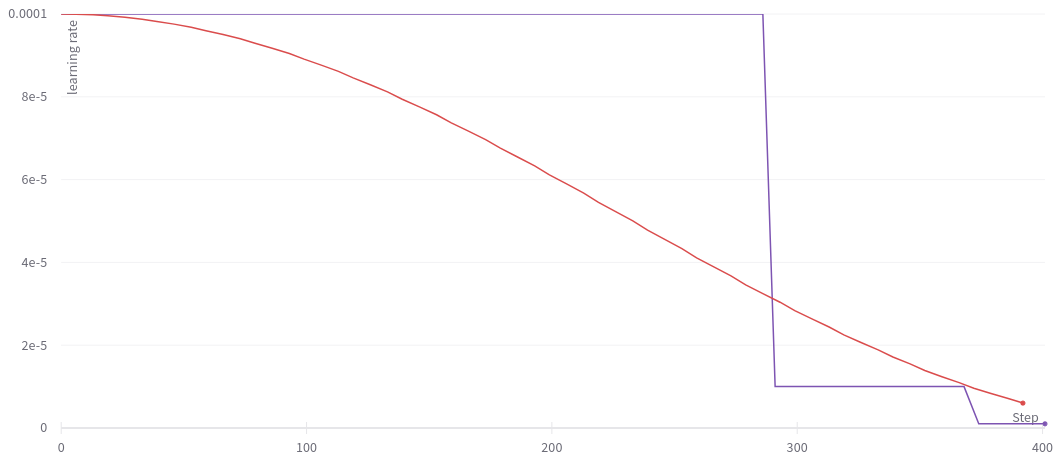
\includegraphics[width=0.5\linewidth]{images/schedulers.png}
    \caption{Learning rate schedulers: Cosine annealing is red, Reduce learning rate on plateau has purple color}
    \label{fig:schedulers}
\end{figure}

\subsubsection{ReduceLROnPlateau}
We couple the scheduler with a model metric, and when the improvement of the metric stalls for a predefined period, the learning rate decreases.
The scheduler is not heavily reliant on the setting of its hyperparameters, making it a go-to starting choice for most developers.

\subsubsection{Cosine annealing}
Cosine annealing changes the value of learning rate according to the equation \ref{eq:cosine_annealing}, where $T$ is half-period of the cosine.
\begin{align}
    lr(t) = lr_{min} + \frac{1}{2} \left( lr_{max} - lr_{min} \right) \left( 1 + \cos \left( \frac{t}{T}\pi \right) \right)
    \label{eq:cosine_annealing}
\end{align}
It is commonly used with two different settings. Either we set $T$ to estimated length of the training. The learning rate than decreases throghout the training, as can be seen in Figure \ref{fig:schedulers}, or we select small value of $T$ and the learning rate oscilates in predefined boundaries multiple times throughout the training. This should help the optimizer to overcome saddle points.

\section{Artificial neural network (ANN)}
The mechanisms of the human brain inspire artificial neural networks. Human neuron cells are in ANN replaced by artificial neurons, which are defined as:
\begin{align}
    y = f \left( \boldsymbol{w}^T \boldsymbol{x}  + b \right).
\end{align}
Where $\boldsymbol{x}$ is a vector of inputs, $\boldsymbol{w}$ stands for weights and $b$ is bias. Symbol $f$ denotes an activation function f : $\mathbb{R} \rightarrow \mathbb{R}$. The artificial neuron proposed by Frank Rosenblatt in the perceptron algorithm worked with a step function \cite{Rosenblatt1958}, but nowadays, different functions such as ReLu, sigmoid or tanh are used. The output of the neuron $y$ is called activation of the neuron.

Neurons are usually structured into layers. The connection between layers depends upon the architectural choice. First ANNs used fully connected layers, meaning that the input into a neuron in layer $n$ was composed of all activations from layer $n-1$. Fully connected neural networks are nowadays sparsely used in computer vision. Convolutional neural networks (CNNs) or vision transformers are used instead. In the case of CNNs we limit neurons' receptive field to the local neighborhood only; this decreases the computation complexity and includes our prior knowledge of pixel neighborhood in the input image. Having the same weights for the whole input makes the network invariant to shifts in the input.

\subsection{Convolutional layer}
A convolutional layer consists of $C_{out}$ neurons, each having $C_{in}, H, W$ receptive field. Those neurons are called kernels with width $W$ height $H$ and several input channels $C_{in}$. In each layer, we convolve\footnote{Even though we usually refer to convolution, in practice, cross-correlation is used instead. Terms cross-correlation and convolution are used interchangeably.} the input $X$  with the kernel $W$, the output $Y$ is defined by:
\begin{align}
    y_{o,i,j} = \sum_{c_{in}} \sum_{\Delta i} \sum_{\Delta j} x_{c, i+\Delta i, j + \Delta j}  w_{o,c, \Delta i, \Delta j}
\end{align}
Nowadays, modifications of convolutional layers are proposed, such as dilated convolution, grouped convolution, or depth-wise separable convolutions are used. However, the fundamentals remain the same: Filter sliding over the input produces an output.

\begin{figure}
    \centering
    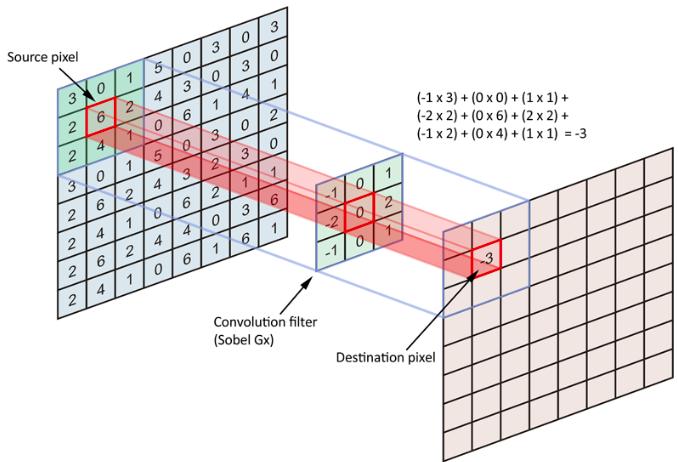
\includegraphics[width=0.9\linewidth]{images/conv_img.png}
\end{figure}

\subsection{Activation functions}
A non-linear activation function usually follows the output of the convolutional layer. Many activation functions are at our disposal, but the most commonly used is ReLU and its derivatives, such as SERLU, SELU, ELU, Swish, and Leaky ReLU. Values of those functions are depicted in Figure \ref{fig:activation_functions}.

\subsection{Normalization layers}
\label{sec:normalization_layers}
Normalization layers make the training of ANNs faster and more stable. It has been shown, that normalization-layers decrease the generalization gap ,while increasing the convergence speed \cite{Ioffe2015,Wu2018}. The normalization layers differ in spatial axis, across which, the normalization statistics is computed, this is illustrated in Figure
\subsubsection{Batch-normalization}
The most normalization layer is batch normalization, which computes the output of the layer $y_i$ as:
\begin{align}
    \hat{x_i} \leftarrow \frac{x_i - \mu_{\mathcal{B}}}{\sqrt{ \sigma _{\mathcal{B}^2} + \epsilon}}; \qquad y_i \leftarrow \gamma \hat{x_i} + \beta
\end{align}
where $\gamma$ and $\beta$ are learnable parameters, $\mathcal{B}$ denotes, that this value is computed over a mini-batch.


\subsubsection{Group-normalization}
\label{sec:group_norm}
Wu et al. \cite{Wu2018} proposed a normalization method, where the statistics are computed over groups of channels. We et al. showed that group normalization outperforms batch normalization when both layers are used with batch sizes smaller than eight.

The disadvantage of group normalization is the introduction of a new group size $G$ hyper-parameter, which needs to be tuned to obtain the results claimed by the authors \cite{Wu2018}.

\begin{figure}
    \begin{floatrow}[2]
        \ffigbox[0.9\FBwidth]{\caption{Graphs of ReLU based activation functions, source \cite{Zhang2018}}\label{fig:activation_functions}}%
        {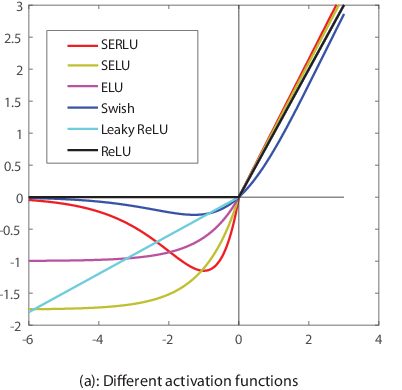
\includegraphics[width=\linewidth]{images/activation_functions.png}}\quad
        \ffigbox[1.1\FBwidth]{\caption{Batch and group normalization layers with denoted axes, across, which the normalization statistics is computed}\label{fig:normalization_layers}}%
        {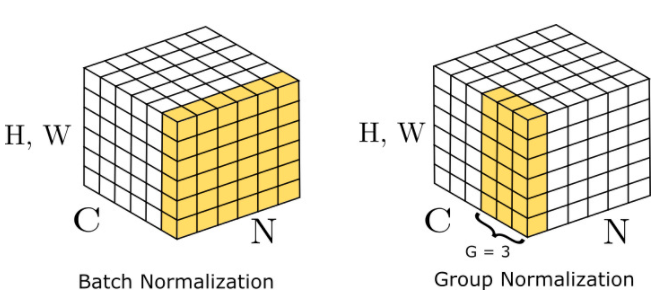
\includegraphics[width=\linewidth]{images/group_batch_norm.png}}
    \end{floatrow}
\end{figure}



\section{Transformer architecture}
Transformer architecture debuted in computer vision in 2021 and has achieved outstanding results, beating state-of-the-art models in multiple benchmarks across all computer vision tasks. As of May 2022, the best-performing models in the main computer vision benchmarks are based on transformer architecture. We think of the following benchmarks to be the main ones in computer vision:  ImageNet benchmark (classification task), COCO (object detection), ADE20K (semantic segmentation).

The transformer architecture was proposed already in 2017 for the task of natural language processing (NLP). We will briefly introduce transformer architecture for the NLP task since it is crucial for understanding transformers for computer vision.

\subsubsection{Transformers in NLP}
Transformer architecture was introduced in the paper Attention is all you need \cite{Vaswani2017} for NLP. NLP is a task where input is a sequence of words of length $n$ and output is a sequence of $m$ words, where $n$ and $m$ usually differ. The sequence of words is converted into a sequence of vectors. There are multiple options for how to embed words into the vector. Commonly used is TD-IDF or Word2Vec\cite{Li2018}. Positional encoding is added to those vectors are then the encoder block processes it. The novel key component is the self-attention module, where for the input sequence of vector values $V$, keys $K$ and queries $Q$ are computed. We output values and keys from the encoder, and from the decoder's self-attention module, we output queries. We then take keys and values from the encoder and queries from the decoder and input them into another attention block:
\begin{align}
    Attention \left(Q,K,V \right) = \text{softmax} \left( \frac{QK^T}{\sqrt{d_k}} \right)V,
\end{align}
where $d_k$ is dimension of keys. More details can be seen in Figure \ref{fig:nlp_transformer} or in \cite{Vaswani2017}.

\begin{figure}
    \centering
    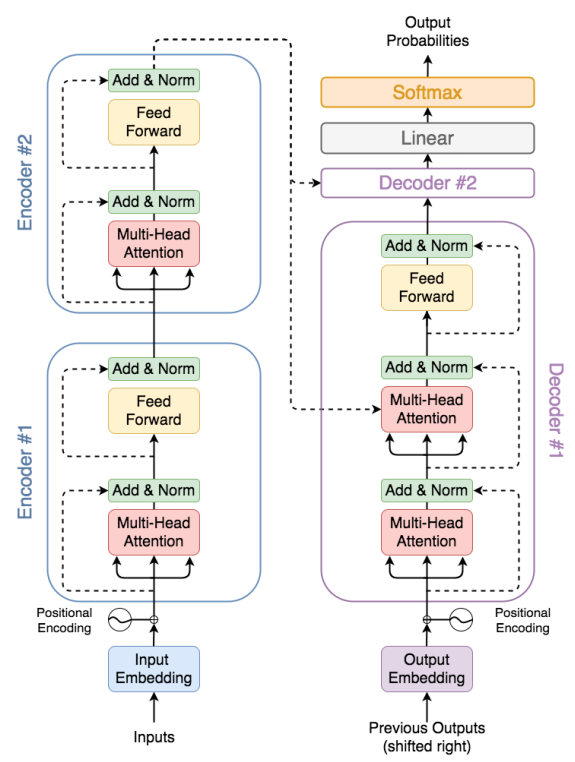
\includegraphics[width=0.5\linewidth]{images/two_layer_transformer.png}
    \caption{Architecture of transformer with two encoders and two decoders, source \cite{Yin2020}}
    \label{fig:nlp_transformer}
\end{figure}

\subsection{Transformers in computer vision}
The first transformer-based model was the Vision Transformer (ViT) which is capable of image classification only. It is composed of multiple encoder blocks stacked on top of each other; those blocks are the same as those used by the transformer for the NLP task. On the top encoder block is attached a multi-layer perceptron (MLP) head, which outputs values for each class. Those can be converted into corresponding probabilities by a softmax layer. The input into ViT are $16 \times 16$ image patches linearly projected into vectors; the whole architecture is shown in Figure
\begin{figure}
    \centering
    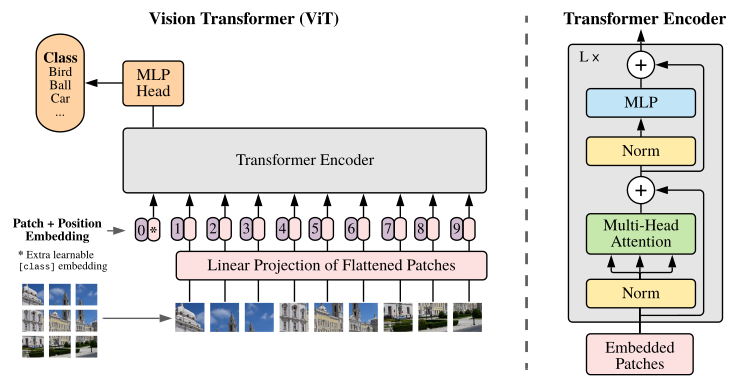
\includegraphics[width=\linewidth]{images/vision_transformer.png}
    \caption{Architecture of ViT, source \cite{Dosovitskiy2020}}
    \label{fig:vision_transformer}
\end{figure}


\section{General architecture for object detection}
Even though there is a wide variety of architectures for object detection, the core principles remain the same. The model is composed of three main parts: backbone, neck, and head, as depicted in Figure \ref{fig:object_detection_architecture}. Each of those blocks can usually be swapped for a different one, fulfilling the same purpose. This gives us great flexibility and allows us to try different combinations of those blocks.



\subsubsection{Backbone}
The purpose of backbones is to transform the input image into feature maps. For this purpose, we use classification models with the classification head removed. Most parameters of object detection models are usually part of the backbone. The extraction of useful feature maps is vital for other blocks to perform well. The most common backbones are models from the ResNet family.

\subsubsection{Neck}
The neck is responsible for the merging of features from the backbone. This is not a straightforward task since we usually use features from different backbone layers. This allows us to get semantically strong features from deeper layers and more detailed information from earlier ones. Common neck architectures are feature pyramid network or PANet \cite{Lin_2017_CVPR}.
\begin{figure}
    \centering
    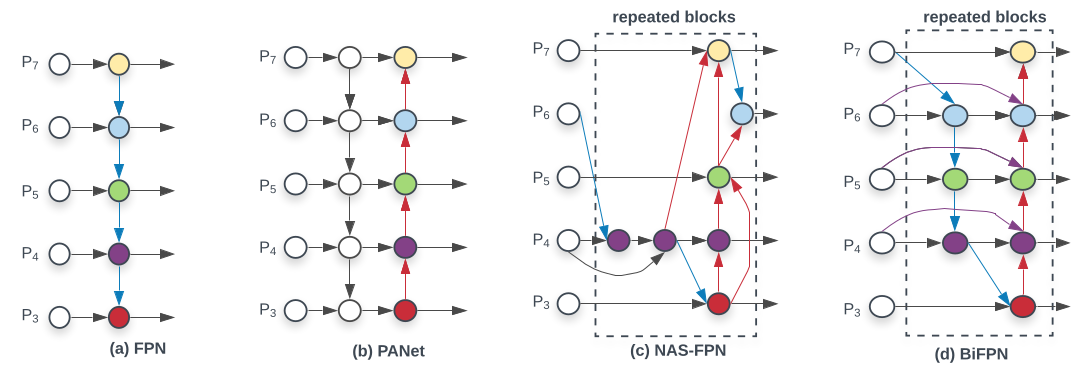
\includegraphics[width=\linewidth]{images/necks_architecture.png}
    \caption{Architecture of different necks for feature fusion, source \cite{Tan2019}}
    \label{fig:necks}
\end{figure}

\subsubsection{Head}
The head is responsible for predicting the position of boxes and their classification. It uses the features extracted by the backbone and merged by the neck. Based on the approach to box prediction, we differ them into Dense prediction heads (YOLO, RetinaNet) or Sparse prediction heads(Faster R-CNN) \cite{Bochkovskiy2020}.


\begin{figure}
    \begin{floatrow}[2]
        \ffigbox[\FBwidth]{\caption{The schema of two-stage detection process of Faster R-CNN }\label{fig:faster_rcnn}}%
        {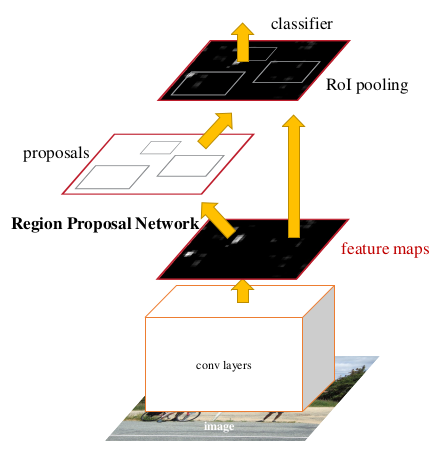
\includegraphics[width=\linewidth]{images/FasterRcnn.png}}\qquad
        \ffigbox[\FBwidth]{\caption{General architecture for object detection, source \cite{Chen2019}}\label{fig:object_detection_architecture}}%
        {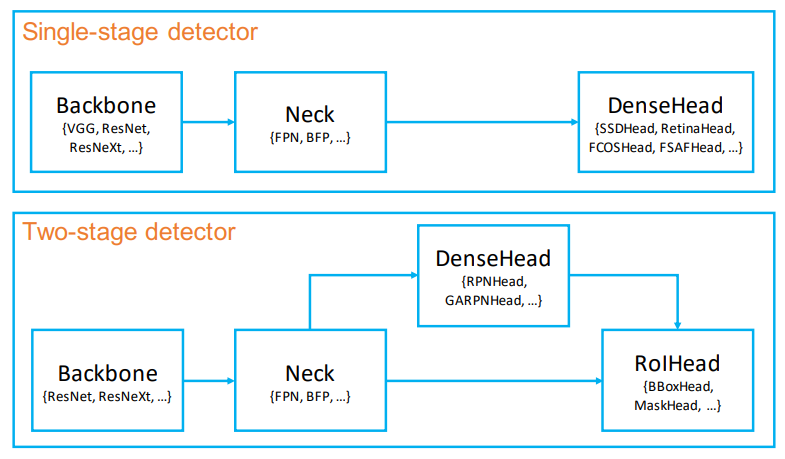
\includegraphics[width=\linewidth]{images/object_detection_architecture.png}}
    \end{floatrow}
\end{figure}

\section{Backbone models}
This section will introduce multiple architectures of neural networks, which were used as a backbone throughout our work.
\subsection{ResNet}
ResNet architecture was introduced by He et al. \cite{He2015} and proposed a novel element of deep-learning architectures - an identity shortcut connection sometimes called a skip-connection. Let $\mathbf{x}$ be the input into a block composed of multiple convolutional layers with activation functions in between\footnote{Addition of batch-normalization, or other layers is possible}; we will call this block a mapping $\mathcal{F}$. The output of the residual block $\mathcal{H}$, derived from $\mathcal{F}$ is defined as:
\begin{align}
    \mathcal{H}\left(\mathbf{x}\right) = \mathcal{F} \left(\mathbf{x}\right) + \mathbf{x}.
\end{align}
The reasoning behind the residual block is to make it easier to learn the identity mapping if desired. This has other benefits, especially the improvement of the gradient flow during back-propagation, making it easier to optimize such blocks. This ease of optimization can be seen by inspecting the loss function landscape of a model with and without skip-connections in Figure \ref{fig:resnet_loss}.
Final ResNet architecture is composed of multiple residual blocks stacked one after another; the models vary in the number of layers used; this is denoted in the name with a number such as ResNet50 or ResNet101.

\begin{figure}
    \centering
    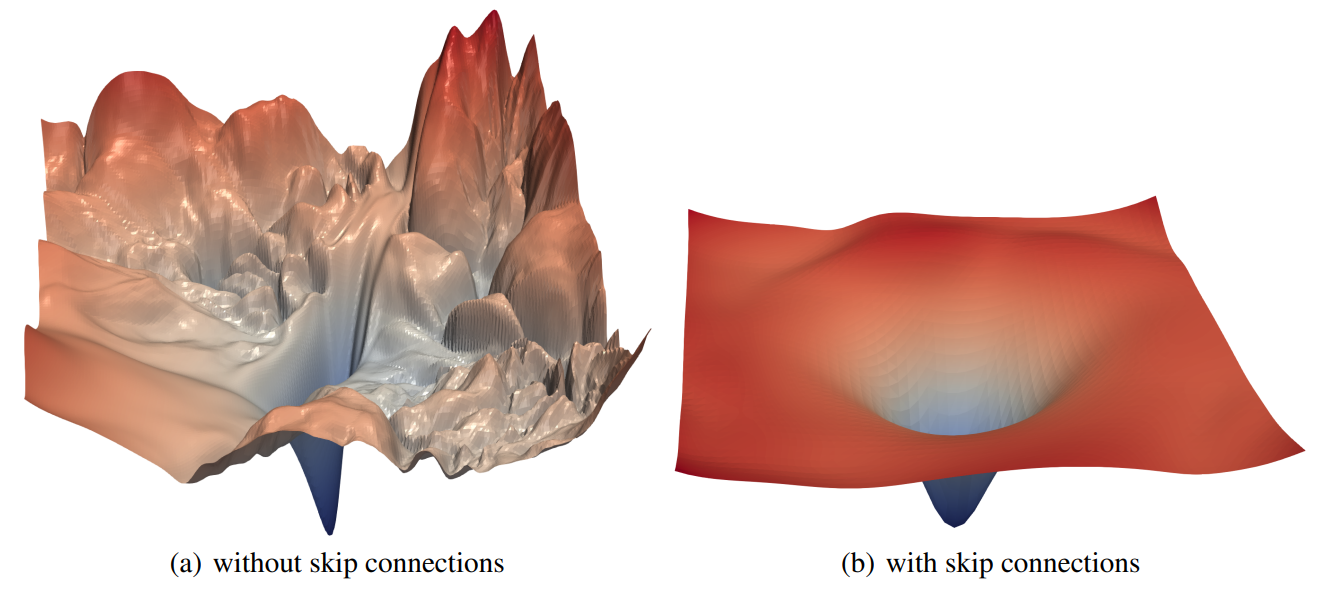
\includegraphics[width=\linewidth]{images/resnet_loss.png}
    \caption{Comparison of loss landscapes, source \cite{Li2017}}
    \label{fig:resnet_loss}
\end{figure}

\subsection{EfficientNet}
When scaling the model's size, we can increase: Number of layers (depth), the number of filters in each layer (width), or the width and height of feature maps (resolution). It has been a common practice to change only one of them. Tan and Le \cite{Tan2019a} did a multi-objective neural network search, where they tried to maximize objective function $O$ defined as:
\begin{align}
    O = ACC \left( m \right) \times \left[ FLOPS \left(m \right) / T \right] ^w,
\end{align}
where $ACC(m)$ and $FLOPS(m)$ are accuracy and floating-point operations (FLOPS) of model $m$, $T$ is the target number of FLOPS, and $w$ is a hyper-parameter controlling the trade-off between accuracy and number of FLOPS of the final model. This search resulted in the EfficientNet-B0 baseline model, which can be scaled to obtain a more extensive network called B1-B7.

\subsection{Swin transformer}
Swin transformer architecture overcomes the limitations of ViT, which is working with $16 \times 16$ image patches only. This is insufficient for segmentation and object detection tasks, where dense predictions are needed. Swin transformers are in the first layer working with $4 \times 4$ patches. Since the computation complexity of the self-attention layer grows quadratically with the number of input tokens, the authors overcome this by using neighbor patches only. Attention is thus computed with respect to tokens in the non-overlapping local window. As depicted in Figure\ref{fig:swin_pathces}, this local window for computing self-attention is shifted after every encoder layer. This shift introduces cross-window connections, which increase the modeling capacity of the model. After a particular number of encoder layers, neighbor patches are merged, which reduces the number of patches while increasing their size by a predefined factor. This mimics the behavior of CNNs, where we start with big, semantically weak feature maps and gradually decrease their dimensions while increasing their number. Having this kind of feature map allows using swin transformer as a general backbone for any task. \cite{Liu2021}

\begin{figure}
    \begin{floatrow}[2]
        \ffigbox[\FBwidth]{\caption{Hierachical structure of Swin Transformer compared with ViT, source \cite{Liu2021}}\label{fig:swin_hierarchy}}%
        {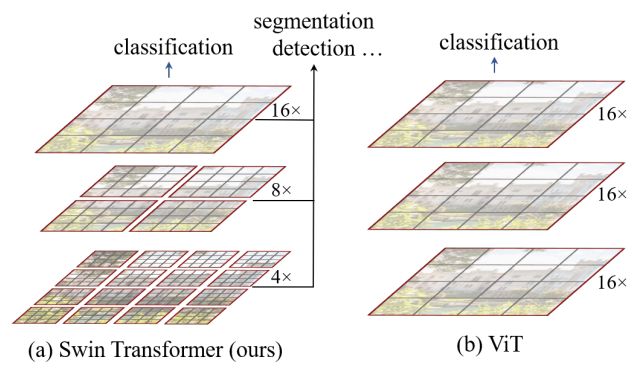
\includegraphics[width=\linewidth]{images/swint_transformer_hierarchy.png}}\qquad
        \ffigbox[\FBwidth]{\caption{Shift of local window for computation of self-attention, source \cite{Liu2021}}\label{fig:swin_pathces}}%
        {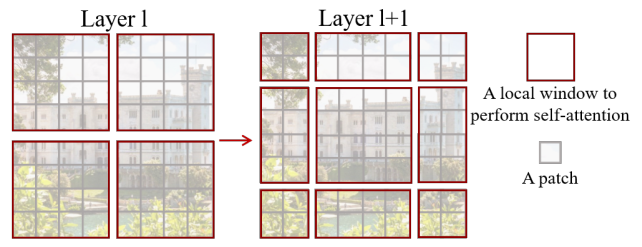
\includegraphics[width=\linewidth]{images/swint_transformer_patches.png}}
    \end{floatrow}
\end{figure}

\section{Detection models}
\label{sec:deteciton_models}

\subsection{Faster R-CNN}
Faster RCNN (Region-Based Neural Network) architecture is a two-stage detector. In the first stage, Region Proposal Network (RPN) finds regions of interest (ROI)and proposes bounding boxes corresponding to those regions. This is done by sliding a small neural network over the output of the backbone. In the second stage, features corresponding to positions of ROIs are extracted from the backbone and processed by a classification network, which decides if the region corresponds to a background or is one of the target classes. The schema of the architecture is in Figure \ref{fig:faster_rcnn}

\subsection{RetinaNet}

\begin{figure}
    \centering
    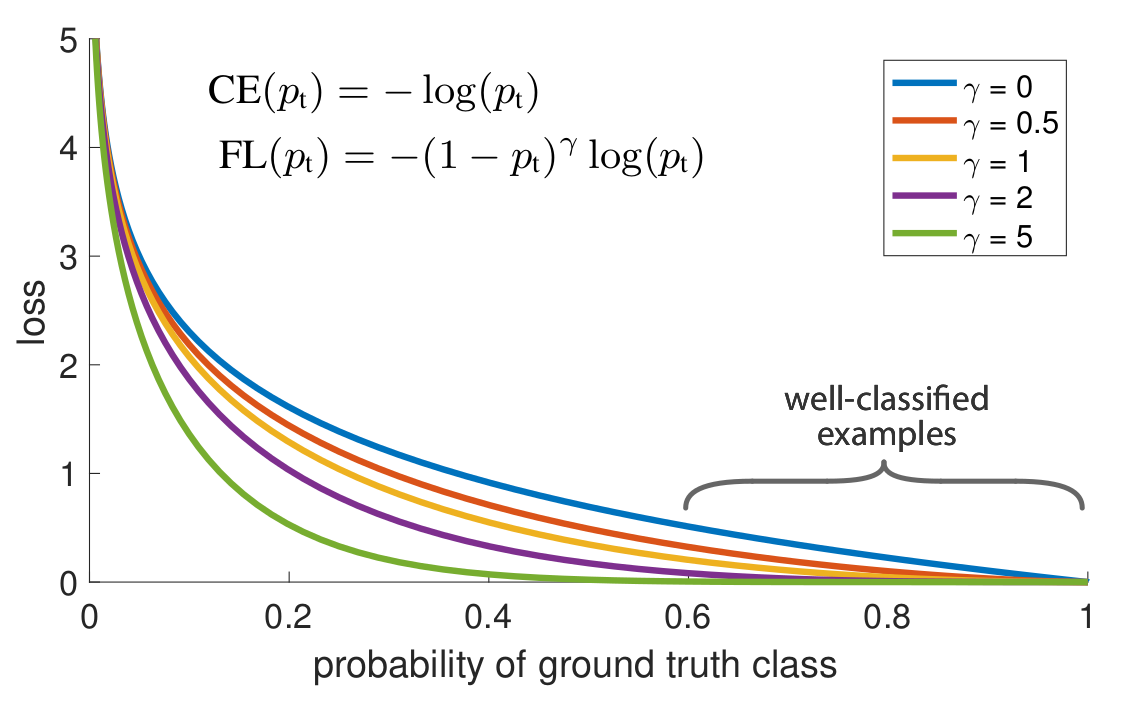
\includegraphics[width=0.7\linewidth]{images/focal_loss.png}
    \caption{Focal Loss, source \cite{Lin2017}}
\end{figure}

\subsection{YOLO family}
TODO

\subsection{EfficientDet}
EfficientDet tries to achieve a similar goal as EfficientNet: Propose a computationally effective architecture for object detection that would be scalable. Since an efficient backbone architecture was already proposed \cite{Tan2019a}, they focus mainly on feature fusion from multiple layers. Based on the study of FPN, PANet, and NAS-FPN, a Bidirectional feature pyramid network (BiFPN) was proposed as the most computationally effective neck architecture \cite{Tan2019}; it consists of multiple BiFPN blocks stacked on top of each other, see \ref{fig:necks}. The count of those blocks is dependent on the size of the used backbone.

\subsection{Models for image segmentation}
\subsubsection{U-Net}
\begin{figure}
    \centering
    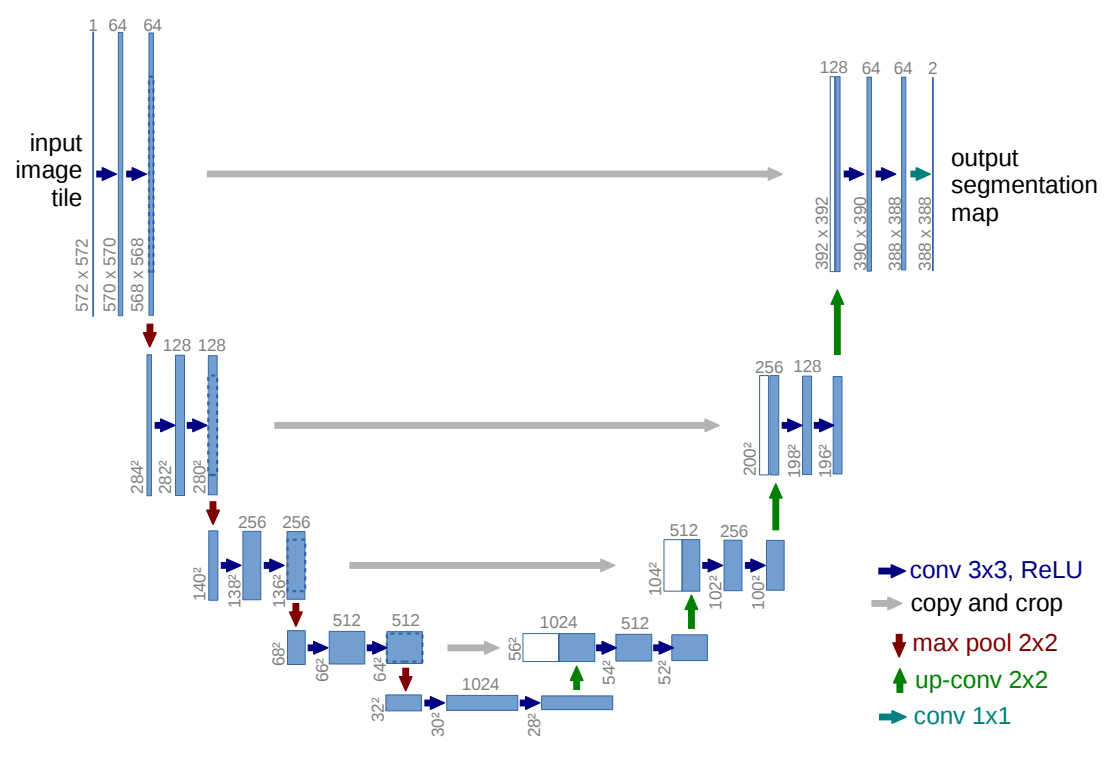
\includegraphics[width=\linewidth]{images/U-Net.png}
    \caption{Architecture of U-Net model, source \cite{Ronneberger2015}}
    \label{fig:unet_architecture}
\end{figure}
U-Net is an architecture for semantic segmentation, with an encoder-decoder structure as shown in Figure \ref{fig:unet_architecture}. The decoder extracts feature maps from the input image with an increasing semantical strength throughout the layers. In the middle of the network is a so-called bottle-neck layer with the strongest semantical information about the image but lacks information about high-resolution details of the input image. Hence when the decoder decodes the information from the bottle neck, it is combined with information from the shallower layer, which contains information about image details required to obtain a precise dense prediction.
\newline
The decoder proposed by Rennenberger et al. \cite{Ronneberger2015} can be replaced by a general-purpose backbone, as demonstrated by Baheti et al. \cite{Baheti2020}, who used EfficientNet as the backbone.

\section{Model ensembling in object detection}
\label{sec:model_ensembling}

Let say we have $M$ different models, each of them predicting $\mathcal{B}_i = \left\{b_1,...,b_N \right\} $ bounding boxes and $\mathcal{S}_i = \left\{ s_1,...,s_N \right\} $ confidence values for a given image corresponding to a single class. We merge predictions of all models together. It is possible to use weights $\mathit{W} = \{w_1,...,w_M \}$ to express our prior belief in the given model. Set of all boxes $\mathcal{B}$ and confidence scores $\mathcal{S}$ is thus obtained by:
\begin{align}
    \mathcal{B} = \bigcup_{i=1}^{M} B_i \quad, \mathcal{S} = \bigcup_{i=1}^{M} \frac{S_i  w_i}{ F},
    \label{eq:ensembling_weighting}
\end{align}
where F is an optional normalization constant. It's only purpose is to ensure that confidence score will be less than 1 after the ensembling. Commonly used value for F is $\frac{1}{M} \sum_{i=1}^M w_i$. After obtaining sets $\mathcal{B}$ and $\mathcal{S}$ we post-process them by one of the following algorithms: Non-maximal suppression, soft non-maximal suppression, non-maximum weighted suppression or weighted boxes fusion.

\subsubsection{Non-maximal supression (NMS)}
In non-maximal suppression, we first sort all boxes $\mathcal{B}$ by their confidence $\mathcal{S}$ in descending order. We go thru the sorted set $\mathcal{B}$ and check if any other box b in $\mathcal{B}$ has an overlap greater than the predefined threshold $N_t$.  In that case, we remove box $b$ from $\mathcal{B}$. More details regarding the NMS algorithm are in the pseudocode, which is in Figure \ref{alg:nms}.
\begin{figure}
    \centering
    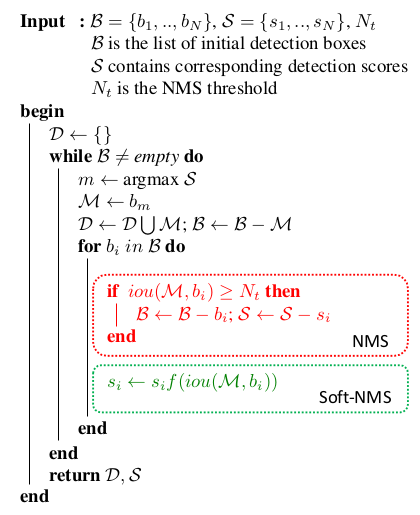
\includegraphics[width=0.5\linewidth]{images/nms_algo.png}
    \caption{Pseud code of NMS and soft-NMS, source \cite{Bodla2017}}
    \label{alg:nms}
\end{figure}

\subsubsection{Soft non-maximal suppression {S-NMS}}
Soft non-maximal supression extends the NMS algorithm by a possibility to keep overlapping the predictions if their confidences are high. Instead of removing boxes with an overlap, we decrease their confidence value by the follwing Gaussian penalty function:
\begin{align}
    s_i = s_i e^{-\frac{\text{iou}\left( \mathcal{M}, b_i \right)^2}{\sigma}}, \forall b_i \notin \mathcal{D}
\end{align}
where $\mathcal{M}$ is the currently processed bounding box, and $\mathcal{D}$ is the set of already processed boxes. After processing all boxes, those with $s_i < T$ are removed, where $T$ stands  for a confidence cut-off threshold \cite{Bodla2017}.

\subsubsection{Non-maximum weighted suppression (NMW)}
Non-maximum weighted suppression does not remove boxes in case of an overlap, but merges them togehter by following formula:
\begin{align}
    \mathcal{M} & = \frac{\sum_{i=1}^n \omega_i \times b_i}{\sum_{i=1}^n \omega_i} \\
    \omega_i    & = s_i \times \text{iou} \left( b_i, b_{ argmax_i s_i} \right)
\end{align}
where $\mathcal{M}$ is the merged bounding box, for which no confidence value is computed \cite{Zhou2017,Solovyev2019}.

\subsubsection{Weighted boxes fusion (WBF)}
Weighted boxes fusion combines boxes similarly to NMW. The main difference is the iterative approach to the fusion, outputting confidence for the merged box, and awareness of several models, which contributed to the prediction.
The steps of WBF are as follows \cite{Solovyev2019}:
\begin{enumerate}
    \item Sort $\mathcal{B}$ by $\mathcal{S}$ as in NMS.
    \item Declare empty lists \boldmath{L} and \boldmath{F} that would be used to store boxes clusters and merged boxes, respectively
    \item Iterate through $\mathcal{B}$. If there is a box in \boldmath{F} for which $IOU > \mathbf{Threshold}$, add the box from $\mathcal{B}$ to list \boldmath{L} on the position corresponding to position of the matched box in \boldmath{F}. If there is no match  found, add it to the end of \boldmath{L}.
    \item Recalculate the box coordinates $\mathcal{M}$ and confidence $c$ in the list \boldmath{F} on the position where we added the box to \boldmath{L} by formulas\ref{eq:wbf1}.
    \item After processing all boxes from $\mathcal{B}$ adjust confidence scores by a formula\ref{eq:wbf2}, where $T$ is the number of contributing boxes and $M$ is the number of models used for ensembling.
\end{enumerate}
\begin{align}
    \mathcal{M} & = \frac{\sum_{i=1}^n c_i \times b_i}{\sum_{i=1}^n c_i} ,\quad c=\frac{\sum_{i=1}^{T}c_i}{T} \label{eq:wbf1} \\
    c           & = c * \frac{T}{M} \label{eq:wbf2}
\end{align}
